\renewcommand{\theequation}{\theenumi}
\begin{enumerate}[label=\arabic*.,ref=\thesubsection.\theenumi]
\numberwithin{equation}{enumi}
\item  given that $\to$
\begin{align}
Z &= x+ 2y
\\
\text{subjected to}
\\
x + 2y &\geq 100
\\
2x - y &\leq 0
\\
2x - y &\leq 200
\\
x  &\geq 0
\\
y &\geq 0
\end{align}
Comparing above equation to the gernelised form$\to$ 
\begin{align}
maxZ &= c^t \vec{x}
\\
\text{subjected to}
\\
A\vec{x} &\preceq b
\\ 
\text{we can find $\to$ }
\\
c &= \myvec{1\\ 2}
\\
A &= \myvec{1 & 2\\2 & -1 \\ 2 & 1}
\\
b &= \myvec{100\\0\\200}
\end{align}\\
Solution for the above equations can be find from the python code of Lenear programing.\\
\begin{lstlisting}
./optimization/codes/lp10.eps
\end{lstlisting}
From the codes we get that the maximum value of the equation will be  at 400 the point (0,200).\\

Maximum value of the equation is 100 but from the line  eqaution 1 we can see that  it gives 100 on each point thus maximum value of function will on the line  $x+2y = 120$ from the point (0,50) to point A.

\begin{figure}[!ht]
	\centering
	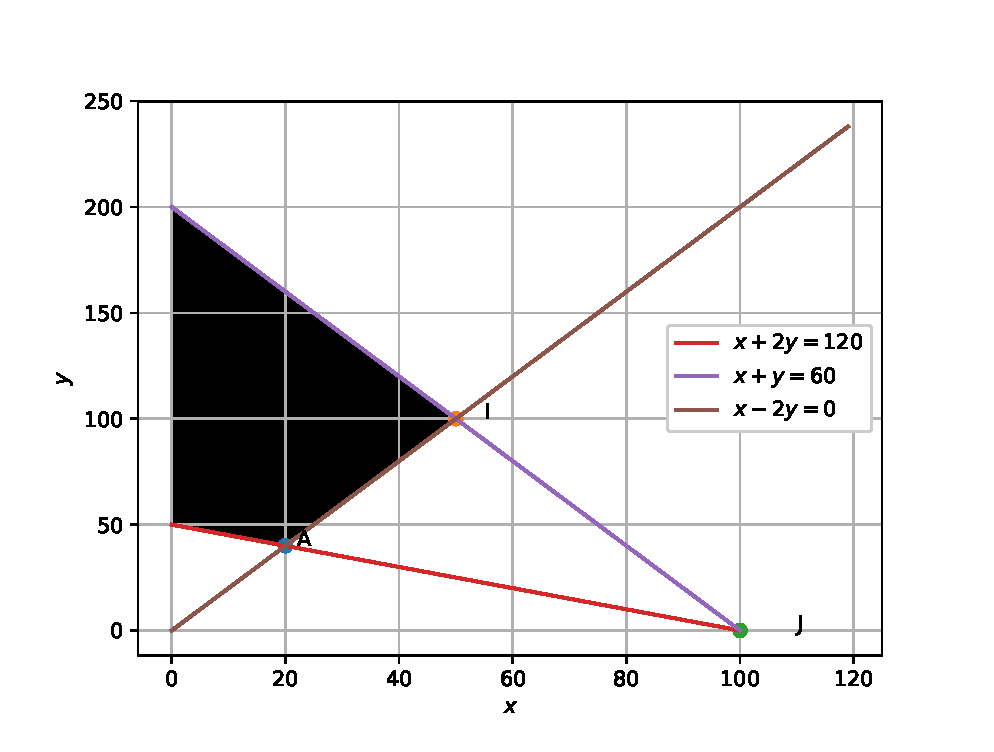
\includegraphics[width=\columnwidth]{./figures/lp10.eps}
	\caption{ lp10}
	\label{fig:lp10}
	pythone codes for the above figure can be get from
	\begin{lstlisting}
	./optimization/figures/lp10.eps
	\end{lstlisting}	
\end{figure}
\end{enumerate}